\documentclass[letterpaper,12pt,fleqn]{article}
\usepackage{matharticle}
\usepackage{tikz}
\usetikzlibrary{positioning}
\usepackage{pgfplots}
\pgfplotsset{compat=1.16}
\usepackage{float}
\renewcommand{\a}{\alpha}
\renewcommand{\l}{\lambda}
\newcommand{\p}{\phi}
\newcommand{\T}{\mathscr{T}}
\renewcommand{\i}{\iota}
\pagestyle{plain}

\begin{document}

\title{Fundamental Groups of Topological Spaces}
\author{Jeffery A. Cavallaro \\ San Jose State University \\ Spring 2020 \\ Math-275a}
\date{11 May 2020}

\maketitle

\section*{Motivation}

To say that two toplogical spaces \(X\) and \(Y\) are \emph{homeomorphic} means that there exists a continuous
bijection \(f:X\to Y\) such that \(f^{-1}\) is also continuous.  Analogous to isomorphic groups, homeomorphic
spaces have the same topological structure.  But as with isomorphic groups, finding a suitable mapping often
proves difficult.  A slightly easier task is to show that two spaces are not homeomorphic by demonstrating that
they differ in some topological property.  One such property is compactness; however, there are some fairly
simple spaces that although compact are not homeomorphic.  Some examples are shown in
\figurename\ \ref{fig:compact}.

\begin{figure}[H]
  \centering
  \begin{minipage}{3in}
    \centering
    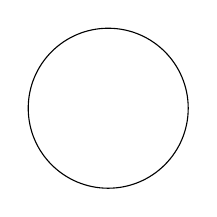
\begin{tikzpicture}
      \draw (0,0) circle [radius=0.4in];
    \end{tikzpicture}

    \(S^1\)
  \end{minipage}
  \begin{minipage}{3in}
    \centering
    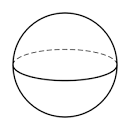
\includegraphics[scale=0.6]{sphere}

    \(S^n\) for \(n\ge2\)
  \end{minipage}

  \begin{minipage}{3in}
    \centering
    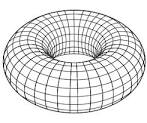
\includegraphics[scale=0.6]{torus}

    \(T=S^1\times S^1\)
  \end{minipage}
  \begin{minipage}{3in}
    \centering
    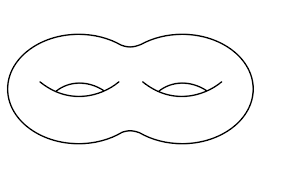
\includegraphics[scale=0.6]{dtorus}

    \(T\#T\)
  \end{minipage}
  \caption{Compact but non-homeomorphic spaces.}
  \label{fig:compact}
\end{figure}

The circle, closed ball, torus, and double torus are all clearly compact; however, they are not homeomorphic.  In
fact, these spaces share most of the standard topological properties, so something different is needed to prove
whether or not they are homeomorphic.  Such a property is the \emph{fundamental group} of a space.  This paper
provides an overview of the fundamental group property of a space and compares the fundamental groups of the
circle, closed ball, torus, and double torus to prove that these spaces are not homeomorphic.

\section*{Homotopy}

The development of the concept of the fundamental group of a space begins with the concept of homotopy.  First, let
\(I=[0,1]\subset\R\), imbued with the subspace topology.  Next, let \(X\) and \(Y\) be topological spaces and let
\(f_1,f_2:X\to Y\) be continuous functions.  To say that \(f_1\) is \emph{homotopic} to \(f_2\), denoted by
\(f_1\simeq f_2\), means that there exists a continuous function \(F:X\times I\to Y\) such that \(F(x,0)=f_1(x)\)
and \(F(x,1)=f_2(x)\).  In particular, if \(f_2\) is a constant function then \(f_1\) is said to be
\emph{nulhomotopic}.

A homotopy can be viewed as a continuous deformation of \(f_1\) into \(f_2\) via a parameterized family of continuous
functions.  The homotopy example shown in \figurename\ \ref{fig:vert} translates a constant function vertically.
Note that by definition, such a constant function is nulhomotopic.

\begin{figure}[H]
  \centering
  \begin{tikzpicture}
    \begin{axis}[
        xmin=0,
        xmax=1,
        ymin=0,
        ymax=1,
        axis lines*=middle,
        xtick={0,1},
        ytick={0,1},
        ytick={0,1/5,2/5,3/5,4/5,1},
        yticklabels={\(0\),\(\frac{1}{5}\),\(\frac{2}{5}\),\(\frac{3}{5}\),\(\frac{4}{5}\),\(1\)},
        xlabel={\(I\)},
        ylabel={\(I\)},
        ylabel style={rotate=-90},
        clip=false
      ]
      \addplot [domain=0:1,red] {0} node [right] {\(f_1(x)=0\)};
      \addplot [domain=0:1,green] {1} node [right] {\(f_2(x)=1\)};
      \addplot [domain=0:1,dashed] {0.2};
      \addplot [domain=0:1,dashed] {0.4};
      \addplot [domain=0:1,dashed] {0.6};
      \addplot [domain=0:1,dashed] {0.8};
    \end{axis}
  \end{tikzpicture}

  \(F(x,t)=\pi_I(x,t)=t\)
  \caption{A vertical translation homotopy.}
  \label{fig:vert}
\end{figure}

The homotopy example shown in \figurename\ \ref{fig:horz} is a horizontal translation.

\begin{figure}[H]
  \centering
  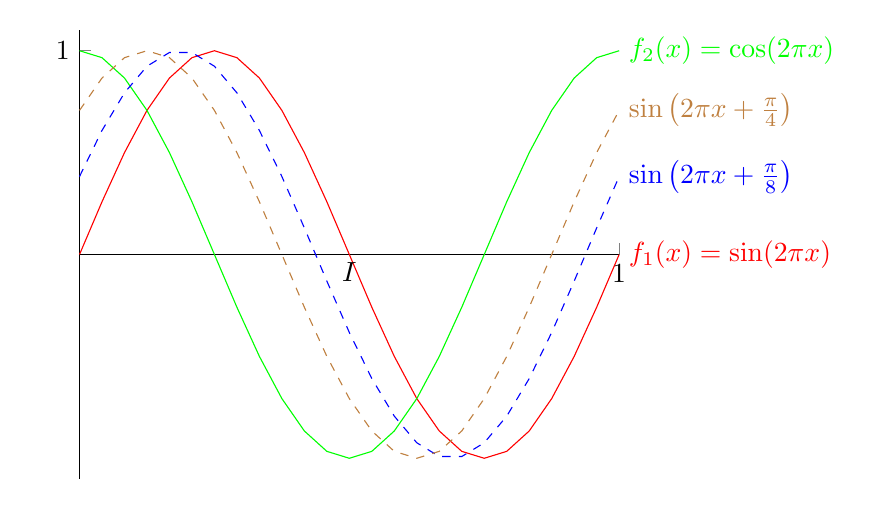
\begin{tikzpicture}
    \begin{axis}[
        xmin=0,
        xmax=1,
        ymin=-1.1,
        ymax=1.1,
        axis lines*=middle,
        xtick={0,1},
        ytick={0,1},
        xlabel={\(I\)},
        ylabel={\(\R\)},
        xlabel style={above=0cm},
        ylabel style={rotate=-90},
        clip=false
      ]
      \addplot [domain=0:1,red] {sin(deg(2*pi*x))} node [right] {\(f_1(x)=\sin(2\pi x)\)};
      \addplot [domain=0:1,green] {cos(deg(2*pi*x))} node [right] {\(f_2(x)=\cos(2\pi x)\)};
      \addplot [domain=0:1,blue,dashed] {sin(deg(2*pi*x+pi/8))}
      node [right] {\(\sin\left(2\pi x+\frac{\pi}{8}\right)\)};
      \addplot [domain=0:1,brown,dashed] {sin(deg(2*pi*x+pi/4))}
      node [right] {\(\sin\left(2\pi x+\frac{\pi}{4}\right)\)};
    \end{axis}
  \end{tikzpicture}

  \(F(x,t)=\sin\left(2\pi x+t\frac{\pi}{2}\right)\)
  \caption{A horizontal translation homotopy.}
  \label{fig:horz}
\end{figure}

And finally, the example shown in \figurename\ \ref{fig:compress} compresses a function into a constant function.
Thus, the former is nulhomotopic.
  
\begin{figure}[H]
  \centering
  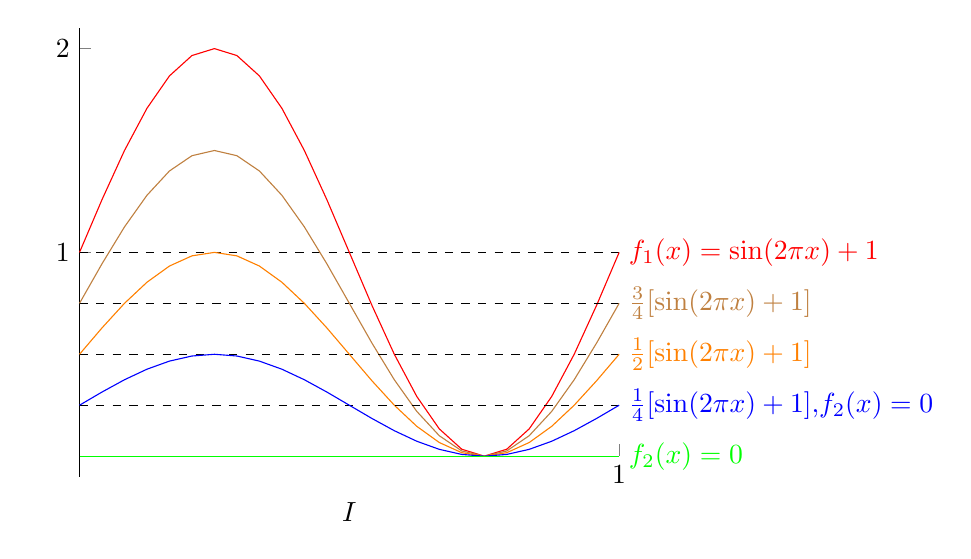
\begin{tikzpicture}
    \begin{axis}[
        xmin=0,
        xmax=1,
        ymin=-0.1,
        ymax=2.1,
        axis lines*=middle,
        xtick={0,1,2},
        ytick={0,1,2},
        xlabel={\(I\)},
        ylabel={\(\R\)},
        ylabel style={rotate=-90},
        clip=false
      ]
      \draw [dashed] (0,1) -- (1,1);
      \addplot [domain=0:1,red] {sin(deg(2*pi*x))+1} node [right] {\(f_1(x)=\sin(2\pi x)+1\)};
      \draw [dashed] (0,3/4) -- (1,3/4);
      \addplot [domain=0:1,brown] {(3/4)*(sin(deg(2*pi*x))+1)} node [right] {\(\frac{3}{4}[\sin(2\pi x)+1]\)};
      \draw [dashed] (0,1/2) -- (1,1/2);
      \addplot [domain=0:1,orange] {(1/2)*(sin(deg(2*pi*x))+1)} node [right] {\(\frac{1}{2}[\sin(2\pi x)+1]\)};
      \draw [dashed] (0,1/4) -- (1,1/4);
      \addplot [domain=0:1,blue] {(1/4)*(sin(deg(2*pi*x))+1)} node [right]
               {\(\frac{1}{4}[\sin(2\pi x)+1]\),\(f_2(x)=0\)};
               \addplot [domain=0:1,green] {0} node [right] {\(f_2(x)=0\)};
    \end{axis}
  \end{tikzpicture}

  \(F(x,t)=(1-t)[\sin(2\pi x)+1]\).
  \caption{A compression homotopy.}
  \label{fig:compress}
\end{figure}

An important property of homotopies is that homotopic is an equivalence relation.  Thus, for topological spaces
\(X\) and \(Y\) and all homotopies between them, \([f]\) denotes the equivalence class of all functions that are
homotopic to \(f\).  A special case occurs when \(Y\) is a convex subset of \(\R^n\) in which any two continuous
functions are homotopic via the so-called \emph{straight-line homotopy}:
\[F(x,t)=(1-t)f_1(x)+tf_2(x)\]
This is demonstrated in \figurename\ \ref{fig:slhomotopy}; corresponding points \(f_1(x)\) and \(f_2(x)\) are
connected by a straight line that is completely contained in \(Y\).

\begin{figure}[H]
  \centering
  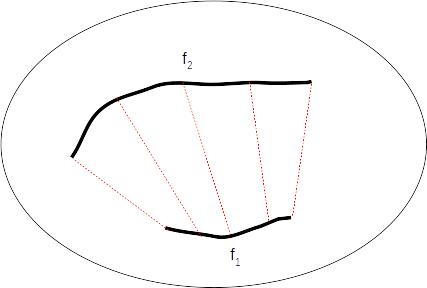
\includegraphics[scale=0.4]{slhomotopy}
  \caption{A straight-line homotopy example}
  \label{fig:slhomotopy}
\end{figure}

\section*{Path Homotopy}

\emph{Path homotopies} are, as the name applies, homotopies between paths.  Given a topological space \(X\), a
path in \(X\) from an initial point \(x_0\) to a final point \(x_1\) is a continuous function \(f:I\to X\) where
\(f(0)=x_0\) and \(f(1)=x_1\).  Thus, a path homotopy between two paths \(f_1,f_2:I\to X\) with the same initial
and final points is a continuous function \(F:X\times I\to X\) such that:

\begin{itemize}
\item \(F(x,0)=f_1(x)\) and \(F(x,1)=f_2(x)\)
\item \(F(0,t)=x_0\) and \(F(1,t)=x_1\)
\end{itemize}

An example of a path homotopy is shown in \figurename\ \ref{fig:path}.

\begin{figure}[H]
  \centering
  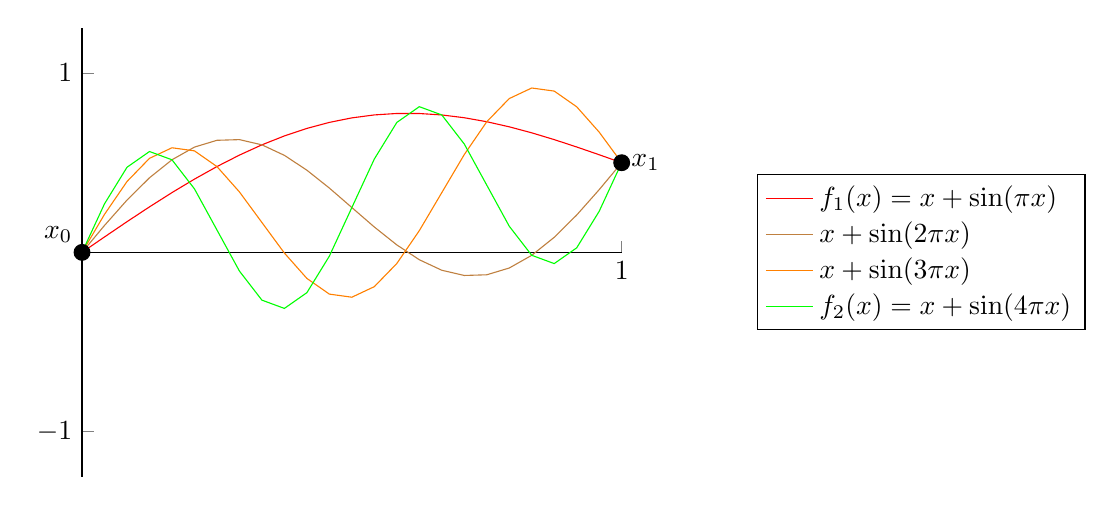
\begin{tikzpicture}
    \begin{axis}[
        xmin=0,
        xmax=1,
        ymin=-2.5,
        ymax=2.5,
        axis lines*=middle,
        xtick={0,1},
        ytick={-2,0,2},
        yticklabels={\(-1\),\(0\),\(1\)},
        legend style={at={(1.25,0.5)},anchor=west},
        legend cell align=left,
        clip=false
      ]
      \addplot [domain=0:1,red] {x+sin(deg(pi*x))};
      \addplot [domain=0:1,brown] {x+sin(deg(2*pi*x))};
      \addplot [domain=0:1,orange] {x+sin(deg(3*pi*x))};
      \addplot [domain=0:1,green] {x+sin(deg(4*pi*x))};
      \node [draw,circle,fill,inner sep=0,minimum size=0.2cm] at (0,0) {};
      \node [above left] at (0,0) {\(x_0\)};
      \node [draw,circle,fill,inner sep=0,minimum size=0.2cm] at (1,1) {};
      \node [right] at (1,1) {\(x_1\)};
      \legend{\(f_1(x)=x+\sin(\pi x)\),\(x+\sin(2\pi x)\),\(x+\sin(3\pi x)\),\(f_2(x)=x+\sin(4\pi x)\)}
    \end{axis}
  \end{tikzpicture}

  \bigskip

  \(F(s,t)=s+\sin[(3t+1)\pi s]\)
  \caption{A path homotopy example.}
  \label{fig:path}
\end{figure}

The equivalence classes of the homotopic paths within a topological space will serve as elements for the
fundamental group.  The next thing that is needed is a binary operator.

\section*{The Product Operator}

Let \(X\) be a topological space.  Let \(f_1\) be a path in \(X\) between initial point \(x_0\) and final point
\(x_1\), and let \(f_2\) be a path in \(X\) between initial point \(x_1\) and final point \(x_2\).  The
\emph{product} of \(f_1\) and \(f_2\), denoted by \(f_1*f_2\), is the path from \(x_0\) to \(x_2\) defined by:
\[f_1*f_2=\begin{cases}
f_1(2t), & t\in\left[0,\frac{1}{2}\right] \\
f_2(2t-1), & t\in\left[\frac{1}{2},1\right] \\
\end{cases}\]
Note that \(f_1*f_2\) is continuous by the pasting lemma.

The product operator is demonstrated in \figurename\ \ref{fig:product}.

\begin{figure}[H]
  \centering
  \begin{tikzpicture}[dot/.style={draw,circle,fill,inner sep=0,minimum size=0.1cm}]
    \node [dot] (X0) at (0,0) {};
    \node [dot] (X1) at (2,1) {};
    \node [dot] (X2) at (4,2) {};
    \draw [blue] (X0) to [bend left] node [above] {\(f_1\)} (X1);
    \draw [green] (X1) to [bend right] node [below] {\(f_2\)} (X2);
    \node [below=1ex of X0] {\(x_0\)};
    \node [below=1ex of X1] {\(x_1\)};
    \node [above=1ex of X2] {\(x_2\)};
  \end{tikzpicture}
  \caption{A product operator example.}
  \label{fig:product}
\end{figure}

Note that when the path equivalence classes of a topological space are paired with the product operator, a so-called
\emph{groupoid} is formed.  The groupoid is not a proper group because the product operator is only a partial
function --- i.e, it is only well-defined when \(f_1(1)=f_2(0)\).  In particular, the groupoid has the following
group-like properties:

\begin{itemize}
\item Associative: \(([f]*[g])*[h]\) is defined if and only if \([f]*([g]*[h])\) is defined and if defined then
  they are equal.
\item Identity: \([e_{x_0}]*[f]=[f]\) and \([f]*[e_{x_1}]=[f]\).
\item Inverse: \([f]*[\bar{f}]=[e_{x_0}]\) and \([\bar{f}]*[f]=[e_{x_1}]\).
\end{itemize}

where \(e_x\) is the \emph{trivial path} that maps \(I\) to the constant value \(x\) and \(\bar{f}(t)=f(1-t)\) is
the reverse path from \(x_1\) to \(x_0\).

\section*{The Fundamental Group}

In order to construct a proper group using the paths in a topological space \(X\) and the product operator, a
single point \(x_0\in X\) is selected.  A path that has \(x_0\) as both its initial and final points is called a
\emph{loop} based at \(x_0\).  The fundamental group for \(X\) is then the homotopic equivalence classes of the
loops based at \(x_0\) paired with the product operator.  Such a group is denoted by \(\pi_1(X,x_0)\).  Note
that \([e_{x_0}]\) is the group identity element and \(\bar{f}\) is the inverse of \(f\).

One might wonder if the fundamental group is dependent on the choice of \(x_0\).  It turns out that for two
different points \(x_0,x_1\in X\), \(\pi_1(X,x_0)\) is isomorphic to \(\pi_1(X,x_1)\).  Thus, although the actual
isomorphism may differ, the structure of the fundamental group is invariant based on the choice of \(x_0\) and
\(x_1\).  Furthermore, if \(\pi_1(X,x_0)\) is not isomorphic to \(\pi_1(Y,y_0)\) then \(X\) and \(Y\) are not
homeomorphic.

An important point to remember is that the fundamental group only describes the connected component containing
\(x_0\).  Thus, fundamental groups are usually only discussed for path connected spaces.

\section*{Simply Connected Spaces}

A special case occurs when the fundamental space for a group is trivial, meaning it consists of the identity
element \([e_{x_0}]\) only.  Such a space is called \emph{simply connected} and is signified as such by the
syntax \(\pi_1(X,x_0)=0\).

Note that due to the straight-line homotopy, any two paths in a convex subspace of \(\R^n\) are homotopic.  Thus,
such spaces are simply connected.  In particular, all open balls (and their closures) in \(\R^n\) are simply
connected: \(\pi_1(B(p,r),x_0)=0\).

\section*{Non-homeomorphic Spaces}

The actual analysis used to determine the fundamental groups of the original four spaces mentioned at the beginning
of this paper is omitted.  However, the results are as follows:

\begin{itemize}
\item \(\pi_1(S^1,x_0)\sim\Z\)

  \begin{center}
    
\begin{tikzpicture}
      \draw (0,0) circle [radius=0.45cm];
    \end{tikzpicture}
  \end{center}

\item \(\pi_1(S^n,x_0)=0\) for \(n\ge2\)

  \begin{center}
    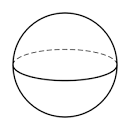
\includegraphics[scale=0.25]{sphere}
  \end{center}

\item \(\pi_1(T=S^1\times S^1,x_0)\sim\Z\times\Z\)\qquad(abelian)

  \begin{center}
    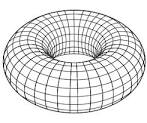
\includegraphics[scale=0.25]{torus}
  \end{center}

\item \(\pi_1(T\#T)\) is not abelian

  \begin{center}
    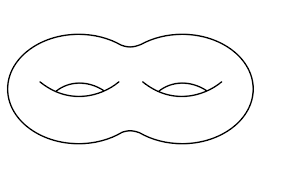
\includegraphics[scale=0.25]{dtorus}
  \end{center}
\end{itemize}

Therefore, since these fundamental groups are not isomorphic, the corresponding spaces are non-homeomorphic.

\newpage

\nocite{*}
\bibliographystyle{amsplain}
\bibliography{fund}

\end{document}
